\documentclass[11pt,a4paper]{article}
\usepackage{graphicx}
\usepackage{float}
\setlength{\textwidth}{6.35in}
\setlength{\oddsidemargin}{0.02in}
\setlength{\evensidemargin}{0.02in}
\setlength{\textheight}{9.25in}
\setlength{\topmargin}{-0.55in}
\setlength{\parindent}{0pt}
\setlength{\parskip}{0.55em}
\setlength{\emergencystretch}{2em}
\renewcommand{\topfraction}{0.9}
\renewcommand{\bottomfraction}{0.8}
\renewcommand{\textfraction}{0.08}
\title{Shared-Gateway ROS 2--REST Performance:\\Actual Source Scaling and Controlled Bottlenecks}
\author{ELEN90061 Communication Networks}
\date{E1 experimental report}
\begin{document}
\maketitle
\begin{abstract}
A shared FIFO ROS 2--REST gateway was evaluated in 35 runs using 1--8 actual source nodes and five repetitions per condition. At eight sources, the reference offered 256.00 messages/s and completed 256.00 requests/s, with a mean run-level successful-message p95 latency of 3.05 ms. At the same offered workload, a 10 ms gateway hold, a 10 ms server hold and a 2 Mbit/s forward-link limit completed 87.15, 87.36, 64.45 requests/s, respectively. Their mean waiting queues were 999.6, 999.7, 999.4 messages, compared with 0.14 in the reference. The restrictions therefore produced upstream application backlog; separate stage timings and CPU measurements distinguish where service time was imposed. A separate 21-run historical loopback rate sweep is retained without pooling cohorts. The results quantify this single-client implementation under controlled conditions, rather than a universal natural-capacity limit.
\end{abstract}
\section{E1: Shared-Gateway Baseline and Controlled Bottleneck Diagnosis}

\subsection{Questions and scope}

This experiment asks whether a shared ROS 2--REST gateway keeps up as the number of actual traffic-source nodes increases, and how a controlled restriction at the gateway, server or network changes its behaviour. The architecture has one HTTP client (the gateway), one server and at most one active HTTP/1.1 request. The TCP connection is reused while healthy; any reconnection is recorded. Increasing ROS 2 source-node count does not increase the number of HTTP clients. All sources are synthetic; no physical robots or external network links are involved.

Two cohorts are reported separately. The historical sweep varied total traffic using at most two ROS 2 nodes over loopback. The revised sweep launches 1, 2, 4 or 8 distinct namespaced ROS 2 source nodes at unchanged per-source rates. All revised conditions use the same isolated virtual-Ethernet (veth) arrangement, with the HTTP server in a separate Linux network namespace. This gives a place to apply a directional rate limit while retaining a common host clock. The revised reference controls the revised diagnostics; it is not a repeat of the historical loopback condition.

\begin{table}[H]
\centering\small
\setlength{\tabcolsep}{4pt}
\begin{tabular}{lrrrr}
\hline
Cohort & ROS 2 sources & Total traffic & Repeats & Timing (s) \\
\hline
Historical loopback & 1 or 2 & 32--2,048/s & 3 & 5 / 60 / 15 \\
Revised reference & 1, 2, 4, 8 & 32--256/s & 5 & 10 / 60 / 30 \\
Revised diagnostics & 8 & 256/s & 5 & 10 / 60 / 30 \\
\hline
\end{tabular}
\caption{Distinct E1 cohorts. Timing denotes warm-up / measurement / maximum drain. Traffic rates include all four message classes.}
\label{tab:e1r-cohorts}
\end{table}


\subsection{Implementation and experimental procedure}

\subsubsection{Topology and workload}

\begin{center}\fbox{\shortstack{1--8 ROS 2\\source nodes}} $\rightarrow$ \fbox{\shortstack{Shared FIFO\\gateway}} $\rightarrow$ \fbox{\shortstack{Isolated veth\\path}} $\rightarrow$ \fbox{\shortstack{HTTP/1.1\\server}}\end{center}

The source nodes share one generator process, publish four class-specific topics each, and feed a single gateway process. The gateway has a FIFO capacity of 1,000 waiting messages, excluding the in-service request; a full queue rejects new arrivals. The server runs in a separate process. HTTP responses acknowledge the unique message identifier. The next request is issued only after the previous response has been read and parsed. The request timeout is 5 s and application retries are disabled.

\begin{table}[H]
\centering\small
\setlength{\tabcolsep}{4pt}
\begin{tabular}{lrrr}
\hline
Class & Messages/s/source & Payload bytes & Deadline ms \\
\hline
command & 2 & 100 & 100 \\
status & 5 & 100 & 200 \\
odometry & 20 & 250 & 100 \\
sensor & 5 & 20,000 & 1,000 \\
\hline
\end{tabular}
\caption{Unchanged traffic per actual ROS 2 source node in the revised experiment. Payload excludes metadata and protocol headers. Deadlines are illustrative project targets.}
\label{tab:e1r-traffic}
\end{table}


Each source produces 32 messages/s and 0.8456 Mbit/s of configured application payload. The four-source and eight-source conditions therefore offer 128 and 256 messages/s; eight sources offer 6.7648 Mbit/s of configured payload. Each source/class stream is periodic after a seeded initial phase. Messages interleave according to their due times and runtime scheduling; there is no fixed repeating class order and no random class selection for each publication. For example, 20 Hz odometry means 50 ms between scheduled publications from one source, not 50 ms of delivery latency; publishing continues while earlier messages wait in the FIFO. Scheduled and actual publication timestamps make source scheduling lag observable.

\subsubsection{Controlled restrictions and repetitions}

\begin{table}[H]
\centering\small
\setlength{\tabcolsep}{4pt}
\begin{tabular}{lrrrr}
\hline
Condition & Actual sources & Gateway hold & Server hold & Forward rate \\
\hline
Reference & 1, 2, 4, 8 & 0 ms & 0 ms & Unshaped \\
Gateway +10 ms & 8 & 10 ms & 0 ms & Unshaped \\
Server +10 ms & 8 & 0 ms & 10 ms & Unshaped \\
Forward 2 Mbit/s & 8 & 0 ms & 0 ms & 2 Mbit/s \\
\hline
\end{tabular}
\caption{Revised matrix: four reference source counts and three single-restriction diagnostics, each repeated five times (35 runs).}
\label{tab:e1r-conditions}
\end{table}


The gateway hold is a sleep after dequeue and before request transmission; it extends serial gateway service time. The server hold is a sleep after parsing the request body and before preparing the acknowledgement. It emulates additional service time, not CPU-intensive server work. The network condition applies a token-bucket rate limit only to gateway egress towards the server. The response direction remains unshaped. The configured burst is 4,000 bytes and the qdisc latency parameter is 200 ms; the latter bounds shaper buffering and is not a fixed propagation delay. No random packet loss or propagation delay is intentionally injected. Network queues may still cause delay or drops under load.

The saved plan shuffles the 35 runs using seed 6106123. Each run warms up for 10 s, measures for 60 s and permits at most 30 s of draining after generation stops. The same workload runs during warm-up and the FIFO is not reset at the measurement boundary. Under deliberate overload it can therefore already be full when measurement begins. Source phases use the saved repetition seed. The nominal measurement duration is 2,100 s in total, excluding warm-up, draining, calibration and setup. Every run saves configuration and code hashes, per-message logs, ROS graph evidence, CPU counters, queue events, network calibration and independent validation. Repeat numbers identify seeded repetitions, not chronological order.

\subsubsection{Timing boundaries and metrics}

All latency timestamps use the same verified Linux monotonic clock, including the server in its network namespace. The endpoint is completion of response-body reading and JSON parsing at the gateway, rather than arrival at the server. For successful messages generated inside the measurement window, the six contiguous intervals are defined in Table~\ref{tab:e1r-stages}. Completions during the bounded drain are included in this latency cohort.

\begin{table}[H]
\centering\small
\setlength{\tabcolsep}{4pt}
\begin{tabular}{lll}
\hline
Interval & Start & Finish \\
\hline
ROS delivery & Before ROS publish & Gateway callback \\
FIFO waiting & Gateway callback & Dequeue \\
Gateway dispatch & Dequeue & Before HTTP request \\
Request to server & Before HTTP request & Body read and parsed \\
Server stage & Body read and parsed & Processing finished \\
Response return & Processing finished & Response read and parsed \\
\hline
\end{tabular}
\caption{Additive latency decomposition. Dispatch includes the hold and serialization. Request-to-server and response-return intervals include software work; neither is pure propagation time. The server stage includes its small receive-to-processing-start gap.}
\label{tab:e1r-stages}
\end{table}


\[L_{\mathrm{total}}=L_{\mathrm{ROS}}+L_{\mathrm{FIFO}}+L_{\mathrm{dispatch}}+L_{\mathrm{request}}+L_{\mathrm{server}}+L_{\mathrm{return}}.\]

The stacked stage figure adds means from exactly the same successful-message cohort, including the small interval between server receive and processing start. The reporting code verifies that the six means sum to the end-to-end mean for every run. Percentiles are calculated separately and are never added. A class p95 is first computed within each run and then averaged across five repetitions; it is not the p95 of pooled messages.

Offered rate counts messages generated inside the measurement window. Admitted rate counts messages from that source-time cohort that enter the FIFO. Throughput and payload goodput instead count successful completions inside the response-time window, so a small difference between offered and completed rates can arise at the boundaries. Payload goodput excludes metadata, HTTP/TCP/IP overhead and responses. A deadline miss includes any generated message that is late or unsuccessful, including FIFO drops, request errors and unresolved work. Queue occupancy is the time integral of waiting-queue length divided by measurement duration. CPU percentages use process CPU-time increments over wall time; 100\% represents one logical CPU. Cumulative CPU counters are sampled every 0.2 s and interpolated at measurement boundaries. Sender occupancy covers dequeue to response completion; handler occupancy covers handler entry to response writing. Occupancy includes sleeping or waiting and differs from CPU use. Points or bar heights are means of five run-level statistics; error bars show the observed minimum and maximum, not confidence intervals.

\subsection{Actual source-node scaling on the reference path}

The source-count sweep holds per-source rates and payloads fixed and changes the number of actual ROS 2 nodes. ROS graph validation confirms the launched nodes and one publisher per expected topic. Figure~\ref{fig:e1r-source-throughput} counts completed responses during each 60 s window and compares them with the configured aggregate arrival rate.

\begin{figure}[H]
\centering
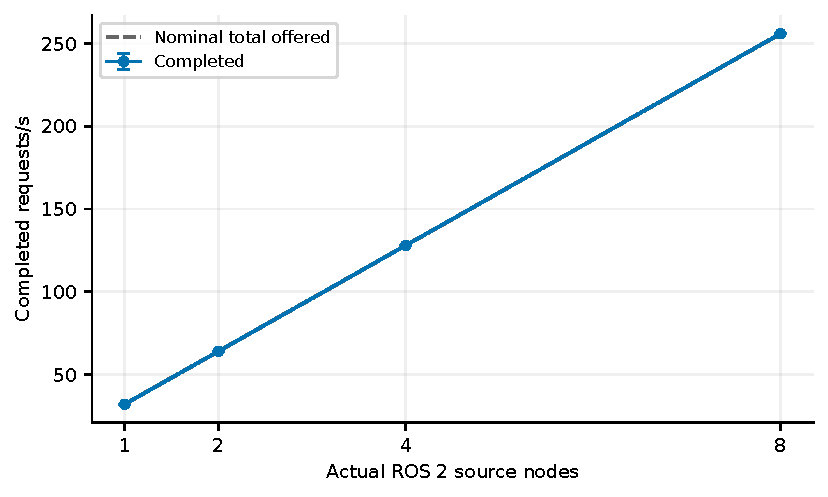
\includegraphics[width=0.88\linewidth]{figures/source_throughput.pdf}
\caption{Reference-path throughput versus actual ROS 2 source nodes. The dashed line is 32 messages/s per source. Points or bar heights are means of five run-level statistics; error bars show the observed minimum and maximum, not confidence intervals.}
\label{fig:e1r-source-throughput}
\end{figure}


Mean completed rates for 1, 2, 4 and 8 actual sources were 32.00, 64.00, 128.00, 256.00 requests/s, respectively. At eight sources, 256.00 messages/s were offered and 256.00 requests/s completed. Across the 20 reference runs, 0 messages were rejected at FIFO admission. This characterises the tested source counts with the shared HTTP connection held fixed.

For Figure~\ref{fig:e1r-source-latency}, successful-message p95 was calculated separately for command, status, odometry and sensor traffic in each run. All four curves at a given source count experience the same mixed workload. The vertical axis shows latency in milliseconds on a linear scale.

\begin{figure}[H]
\centering
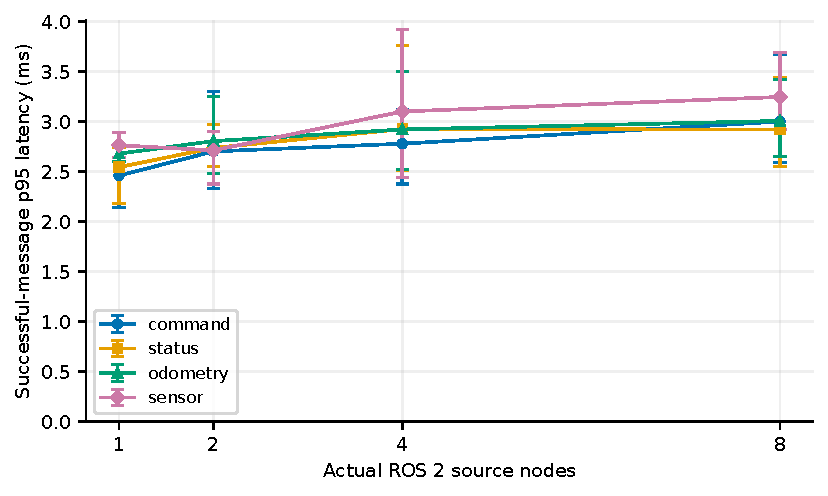
\includegraphics[width=0.88\linewidth]{figures/source_latency.pdf}
\caption{Class-specific p95 latency on the reference path. Each curve represents one class within the same mixed traffic. Successful messages only. Points or bar heights are means of five run-level statistics; error bars show the observed minimum and maximum, not confidence intervals.}
\label{fig:e1r-source-latency}
\end{figure}


At eight sources, mean run-level p95 values were command 3.00 ms, status 2.92 ms, odometry 3.01 ms, sensor 3.25 ms. The mean command deadline-miss percentage was 0.00\%. Latency describes only successful messages; deadline failures and drops must also be considered before judging timeliness.

Figure~\ref{fig:e1r-source-cpu} uses process CPU counters to distinguish source generation, gateway work and server work. Its x-axis denotes actual ROS 2 nodes, all of which share the source process.

\begin{figure}[H]
\centering
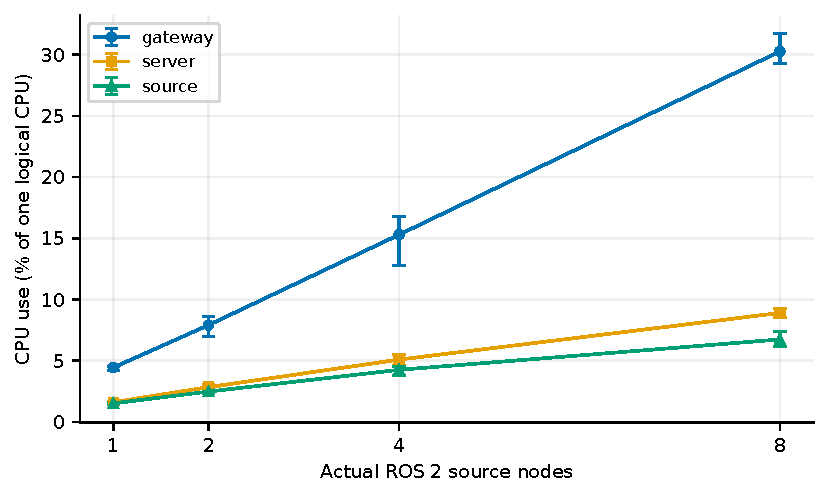
\includegraphics[width=0.88\linewidth]{figures/source_cpu.pdf}
\caption{Process CPU consumption on the reference path, normalised to one logical CPU. Points or bar heights are means of five run-level statistics; error bars show the observed minimum and maximum, not confidence intervals.}
\label{fig:e1r-source-cpu}
\end{figure}


At eight sources, source, gateway and server CPU consumption averaged 6.74\%, 30.27\%, 8.91\% of one logical CPU, respectively. These measurements describe demand on this shared host; they do not by themselves establish the maximum sustainable source count.

\clearpage\subsection{Locating the effect of a controlled restriction}

The following comparisons hold eight actual sources, their mixed traffic and the veth topology fixed. Each diagnostic changes one restriction. The eight-source reference is therefore the appropriate control for these comparisons.

Figure~\ref{fig:e1r-diagnostic-throughput} divides completed requests by the 60 s window. A 10 ms hold on a serial path alone gives an ideal ceiling of 100 requests/s before other service costs; a 2 Mbit/s limit constrains bytes rather than requests. Because messages differ in size and admission drops can change the delivered class mix, a byte-rate limit cannot be converted to a request capacity using one fixed message size.

\begin{figure}[H]
\centering
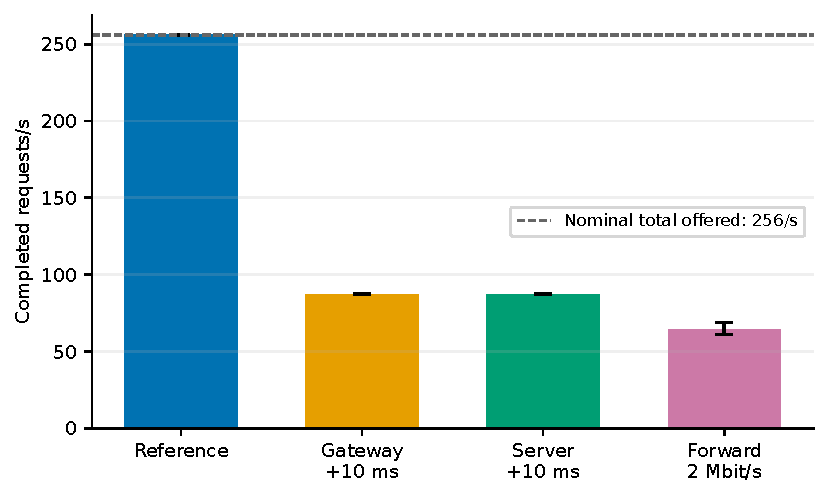
\includegraphics[width=0.88\linewidth]{figures/diagnostic_throughput.pdf}
\caption{Throughput at eight actual sources (nominal aggregate rate 256 messages/s). Points or bar heights are means of five run-level statistics; error bars show the observed minimum and maximum, not confidence intervals.}
\label{fig:e1r-diagnostic-throughput}
\end{figure}


Mean completed throughput was reference: 256.00 requests/s; gateway +10 ms: 87.15 requests/s; server +10 ms: 87.36 requests/s; forward 2 Mbit/s: 64.45 requests/s. These values measure the deliberate restrictions under a fixed workload. They are not universal capacities of HTTP/1.1, ROS 2 or the host.

\begin{table}[H]
\centering\small
\setlength{\tabcolsep}{4pt}
\begin{tabular}{lrrrrr}
\hline
Condition & Mb/s & Drop \% & Cmd miss \% & Sender \% & Handler \% \\
\hline
Reference & 6.76 & 0.00 & 0.00 & 20.60 & 8.55 \\
Gateway +10 ms & 1.96 & 65.95 & 100.00 & 99.85 & 2.68 \\
Server +10 ms & 1.96 & 65.87 & 100.00 & 99.82 & 93.81 \\
Forward 2 Mbit/s & 1.63 & 74.83 & 100.00 & 99.90 & 94.32 \\
\hline
\end{tabular}
\caption{Supporting diagnostic means at eight sources. Mb/s denotes delivered application payload; drops denote FIFO admission losses. Command misses include unsuccessful messages. Activity fractions are wall-time occupancy, not CPU percentages.}
\label{tab:e1r-diagnostic-metrics}
\end{table}


Figure~\ref{fig:e1r-diagnostic-queue} integrates event-based waiting-queue occupancy. It measures work waiting before transmission, which packet timing alone cannot recover.

\begin{figure}[H]
\centering
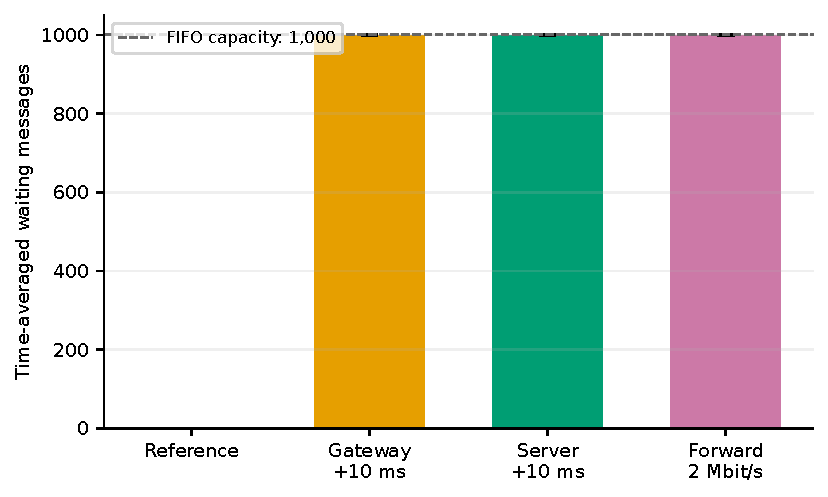
\includegraphics[width=0.88\linewidth]{figures/diagnostic_queue.pdf}
\caption{Mean FIFO occupancy at eight sources, excluding the in-service request. The dashed line marks capacity. Points or bar heights are means of five run-level statistics; error bars show the observed minimum and maximum, not confidence intervals.}
\label{fig:e1r-diagnostic-queue}
\end{figure}


Mean queue occupancies were reference: 0.14 messages; gateway +10 ms: 999.65 messages; server +10 ms: 999.66 messages; forward 2 Mbit/s: 999.42 messages. Because warm-up backlog carries into measurement, a nearly full mean queue can describe sustained overload rather than growth from an empty queue. It indicates that the serial path is not draining arrivals fast enough; this symptom alone does not identify the restricting stage.

Figure~\ref{fig:e1r-diagnostic-latency} calculates successful-message p95 separately by class and repetition. FIFO retains arrival order, so a restriction affecting a long sensor transfer can also delay a later short command.

\begin{figure}[H]
\centering
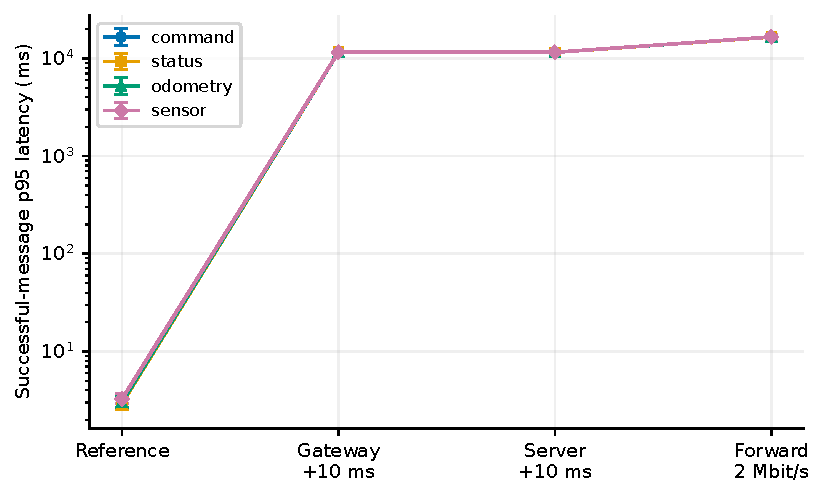
\includegraphics[width=0.88\linewidth]{figures/diagnostic_latency.pdf}
\caption{Per-class successful-message p95 at eight sources. The vertical axis is logarithmic. Points or bar heights are means of five run-level statistics; error bars show the observed minimum and maximum, not confidence intervals.}
\label{fig:e1r-diagnostic-latency}
\end{figure}


Command mean run-level p95 was reference: 3.00 ms; gateway +10 ms: 11,588.00 ms; server +10 ms: 11,552.07 ms; forward 2 Mbit/s: 16,569.59 ms. Queue and deadline measurements distinguish delay among survivors from messages that never completed.

All four classes had zero deadline failures in every one of the 20 reference runs. Conversely, every class had 100\% deadline failures in all 15 restricted runs. Thus the restrictions affected timeliness across the entire FIFO mix, including messages that were eventually delivered successfully.

Figure~\ref{fig:e1r-diagnostic-stages} averages each contiguous interval over successful messages in each run, then averages the five run means. The stack height is the corresponding mean end-to-end latency. When FIFO waiting dominates, small service intervals are hard to see at this scale; Table~\ref{tab:e1r-small-stages} retains their numerical values without removing the queue contribution.

\begin{figure}[H]
\centering
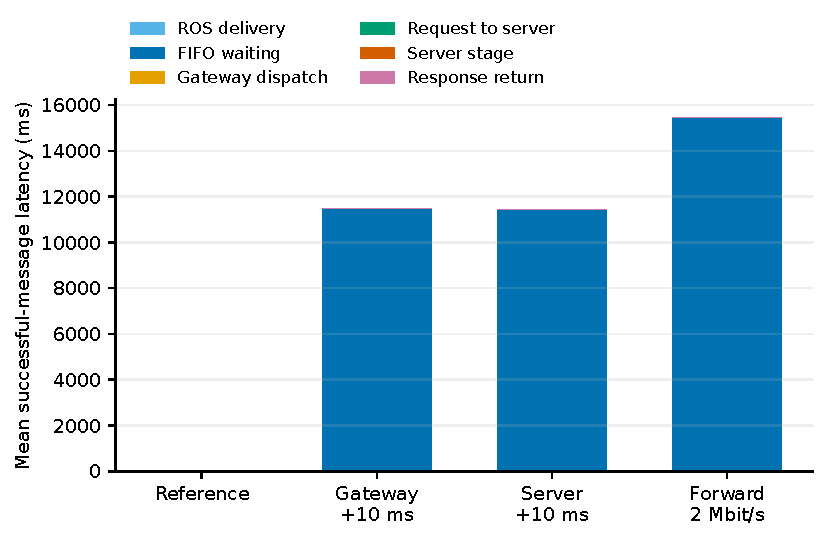
\includegraphics[width=0.88\linewidth]{figures/diagnostic_stages.pdf}
\caption{Additive mean latency for successful measurement-cohort messages, including drain completions. Components average five run means. These are not p95 components; no stacked error bars are inferred from component ranges.}
\label{fig:e1r-diagnostic-stages}
\end{figure}


\begin{table}[H]
\centering\small
\setlength{\tabcolsep}{4pt}
\begin{tabular}{lrrrr}
\hline
Condition & Dispatch ms & Request ms & Server ms & Return ms \\
\hline
Reference & 0.029 & 0.446 & 0.002 & 0.328 \\
Gateway +10 ms & 10.461 & 0.525 & 0.003 & 0.467 \\
Server +10 ms & 0.035 & 0.413 & 10.368 & 0.608 \\
Forward 2 Mbit/s & 0.030 & 14.902 & 0.003 & 0.430 \\
\hline
\end{tabular}
\caption{Service-path means from the same successful cohort as the stacked figure. Dispatch includes serialization and any gateway hold; the server stage includes its small pre-processing gap.}
\label{tab:e1r-small-stages}
\end{table}


For gateway +10 ms, the gateway dispatch interval averaged 10.461 ms, compared with 0.029 ms in the reference. This is a measured service-path component; its upstream waiting consequences are separately visible in the stack.

For server +10 ms, the server stage interval averaged 10.368 ms, compared with 0.002 ms in the reference. This is a measured service-path component; its upstream waiting consequences are separately visible in the stack.

For forward 2 Mbit/s, the request to server interval averaged 14.902 ms, compared with 0.446 ms in the reference. This is a measured service-path component; its upstream waiting consequences are separately visible in the stack.

Figure~\ref{fig:e1r-diagnostic-cpu} reports CPU consumption under the same restrictions. Sleeping for 10 ms or waiting for the network can occupy a service slot without consuming a CPU throughout that interval.

\begin{figure}[H]
\centering
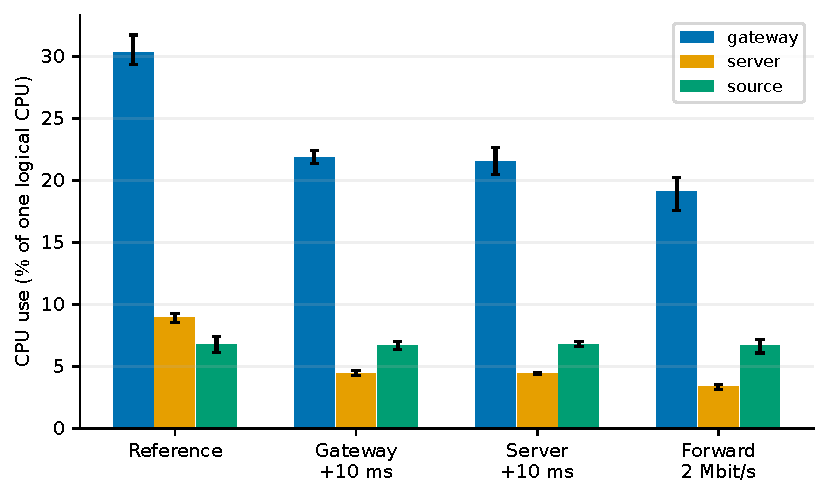
\includegraphics[width=0.88\linewidth]{figures/diagnostic_cpu.pdf}
\caption{Process CPU consumption under controlled restrictions at eight sources. Bars average five runs; error bars show observed minima and maxima. CPU is normalised to one logical CPU.}
\label{fig:e1r-diagnostic-cpu}
\end{figure}


With the server hold, server CPU averaged 4.43\%, while the handler was occupied for 93.81\% of the window. The experiment imposes server service time through sleeping and does not demonstrate CPU saturation.

\begin{table}[H]
\centering\small
\setlength{\tabcolsep}{4pt}
\begin{tabular}{p{0.16\linewidth}p{0.31\linewidth}p{0.43\linewidth}}
\hline
{\raggedright Intervention\par} & {\raggedright Observed evidence\par} & {\raggedright Interpretation and limit\par} \\
\hline
{\raggedright Reference path\par} & {\raggedright Eight-source throughput 256.00/s; mean queue 0.14.\par} & {\raggedright Tests actual source scaling without an imposed hold or rate cap. It does not establish the natural maximum service capacity.\par} \\
{\raggedright Gateway hold\par} & {\raggedright Dispatch 10.461 ms; sender occupied 99.85\%.\par} & {\raggedright The hold extends serial service. This is not evidence of gateway CPU exhaustion.\par} \\
{\raggedright Server hold\par} & {\raggedright Server stage 10.368 ms; server CPU 4.43\%.\par} & {\raggedright The added service interval is measured. Sleeping does not model CPU-bound processing.\par} \\
{\raggedright Forward limit\par} & {\raggedright Bulk calibration 1.91--1.92 Mbit/s.\par} & {\raggedright Forward bandwidth is verified separately. REST goodput also depends on overhead, serial requests and delivered traffic mix.\par} \\
{\raggedright Historical overload\par} & {\raggedright At nominal 2,048/s: queue 999.69; gateway CPU 114.17\%.\par} & {\raggedright Consistent overflow and occupied serial sender implicate the client path. Shared-host variability prevents a stable natural-capacity or CPU-causation claim.\par} \\
\hline
\end{tabular}
\caption{Diagnosis combines the manipulated condition with measured stages. Similar queue and latency symptoms alone do not identify a bottleneck.}
\label{tab:e1r-evidence}
\end{table}


\begin{table}[H]
\centering\small
\setlength{\tabcolsep}{4pt}
\begin{tabular}{lrrrr}
\hline
Condition & Sender \% & Dispatch \% & Handler \% & Processing \% \\
\hline
Reference & 20.60 & 0.75 & 8.55 & 0.01 \\
Gateway +10 ms & 99.85 & 91.15 & 2.68 & 0.01 \\
Server +10 ms & 99.82 & 0.30 & 93.81 & 90.59 \\
Forward 2 Mbit/s & 99.90 & 0.19 & 94.32 & 0.00 \\
\hline
\end{tabular}
\caption{Occupied-time means over five runs. Sender is dequeue to response completion; dispatch is dequeue to request start; handler includes waiting for the request body; processing is the explicit server processing interval. These overlap and must not be added.}
\label{tab:e1r-activity}
\end{table}


Under the forward rate limit, server-handler occupancy averaged 94.32\%, while explicit server-processing occupancy averaged 0.0044\%. The handler starts before the full request body has arrived, so a high handler occupancy can reflect waiting for a shaped upload. It is not sufficient evidence of a server-processing or CPU bottleneck. The measured request interval, processing interval, CPU and calibrated path must be interpreted together.

\clearpage\subsection{Historical aggregate-load sweep: separate loopback evidence}

The original 21 runs are retained as evidence about increasing aggregate traffic through a shared gateway. There was one source node at 32 messages/s and two at the higher tested rates; the two nodes published faster as total offered traffic increased. Tested totals were 32, 64, 128, 256, 512, 1,024 and 2,048 messages/s. These were generated messages and measured outcomes, not extrapolated points. They do not represent that many independent clients or a sweep of actual source counts. These runs used loopback, a 5 s warm-up, 60 s measurement, up to 15 s drain and three repetitions. Their values are not pooled with the new veth measurements or presented as a before/after optimisation comparison.

\subsubsection{Completed throughput}

Completed responses inside each measurement window were divided by 60 s. The horizontal axis is the measured total generated rate across all four classes.

\begin{figure}[H]
\centering
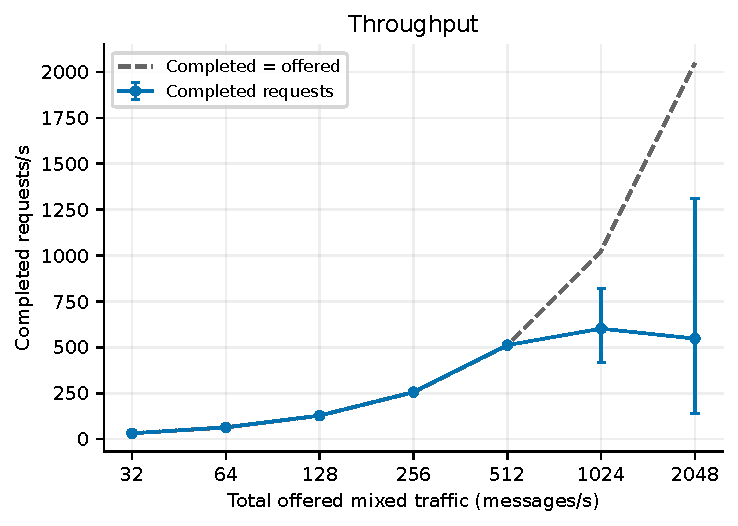
\includegraphics[width=0.88\linewidth]{figures/historical_fig4_throughput.pdf}
\caption{Historical loopback throughput versus total offered mixed traffic. Points average three runs; bars show minimum--maximum. The reference line denotes completed rate equal to offered rate.}
\label{fig:e1r-historical-fig4-throughput}
\end{figure}


At nominal 512 messages/s, mean completed throughput was 512.1 requests/s; at nominal 2,048/s it was 547.5 requests/s. The shared path fell behind the high-load traffic.

\subsubsection{Queue accumulation}

Queue occupancy was integrated from event timestamps and excludes the in-service request.

\begin{figure}[H]
\centering
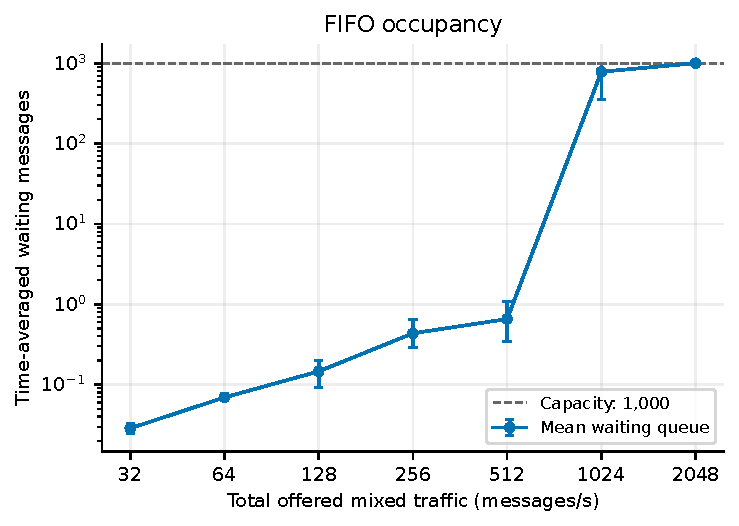
\includegraphics[width=0.88\linewidth]{figures/historical_fig3_queue.pdf}
\caption{Historical loopback mean FIFO occupancy versus total offered mixed traffic. Points average three runs; bars show minimum--maximum.}
\label{fig:e1r-historical-fig3-queue}
\end{figure}


Mean occupancy rose from 0.65 messages at nominal 512/s to 999.69 at nominal 2,048/s, against a capacity of 1,000. This is application backlog, not a router-queue measurement.

\subsubsection{Consequences for latency}

Each curve is one class's successful-message p95 under the same combined traffic. The total-rate coordinate is not that class's individual publishing rate.

\begin{figure}[H]
\centering
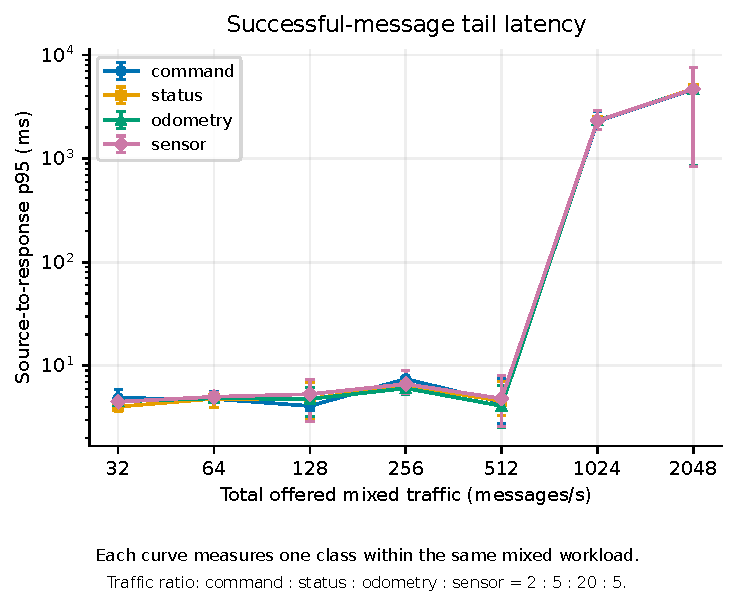
\includegraphics[width=0.88\linewidth]{figures/historical_fig1_latency.pdf}
\caption{Historical loopback per-class source-to-response p95. Points average three run-level p95 values; bars show minimum--maximum. Successful measurement-cohort messages include bounded-drain completions.}
\label{fig:e1r-historical-fig1-latency}
\end{figure}


Mean odometry p95 rose from 4.10 ms at nominal 512/s to 4,691.65 ms at nominal 2,048/s. Increased waiting affects all FIFO classes.

\subsubsection{Consequences for deadlines}

Deadline-failure fractions include late successful messages and unsuccessful generated messages, including overflow drops. The denominator is all generated messages of the class during measurement.

\begin{figure}[H]
\centering
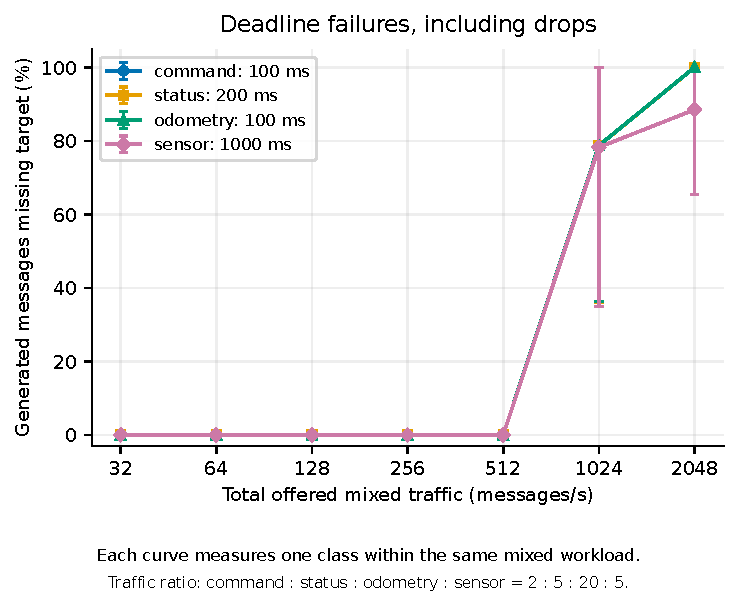
\includegraphics[width=0.88\linewidth]{figures/historical_fig2_deadlines.pdf}
\caption{Historical loopback class-specific deadline-failure percentages. Points average three run percentages; bars show minimum--maximum. Targets are shown in the legend.}
\label{fig:e1r-historical-fig2-deadlines}
\end{figure}


At nominal 2,048/s, command deadline failures averaged 100.00\%. Low latency among delivered survivors would therefore be insufficient evidence of acceptable service.

\subsubsection{Resource demand}

Process CPU time was measured over the same window; 100 percent denotes one logical CPU.

\begin{figure}[H]
\centering
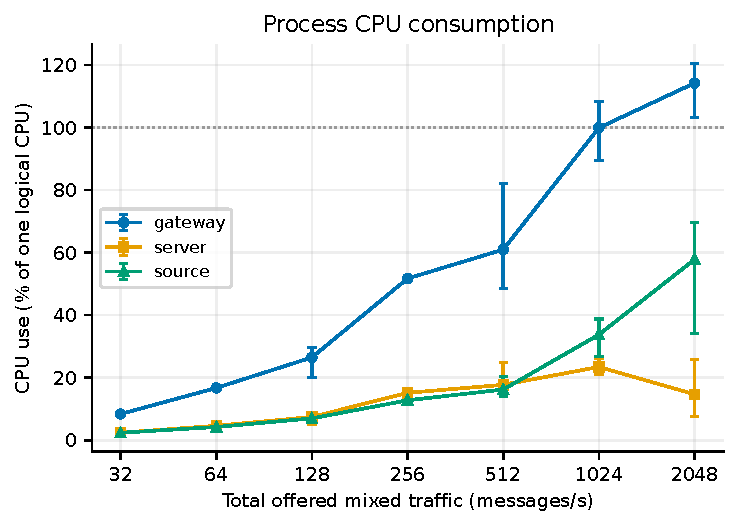
\includegraphics[width=0.88\linewidth]{figures/historical_fig5_cpu.pdf}
\caption{Historical loopback process CPU consumption. Points average three runs; bars show minimum--maximum. Multithreaded process CPU can exceed 100 percent.}
\label{fig:e1r-historical-fig5-cpu}
\end{figure}


At nominal 2,048/s, gateway CPU averaged 114.2\%, compared with 14.7\% at the server. The measurements implicate the gateway/client path but do not establish saturation of a physical network link.

\subsubsection{Occupied time versus CPU}

The sender interval covers dequeue through response parsing; the handler interval covers handler entry through response writing.

\begin{figure}[H]
\centering
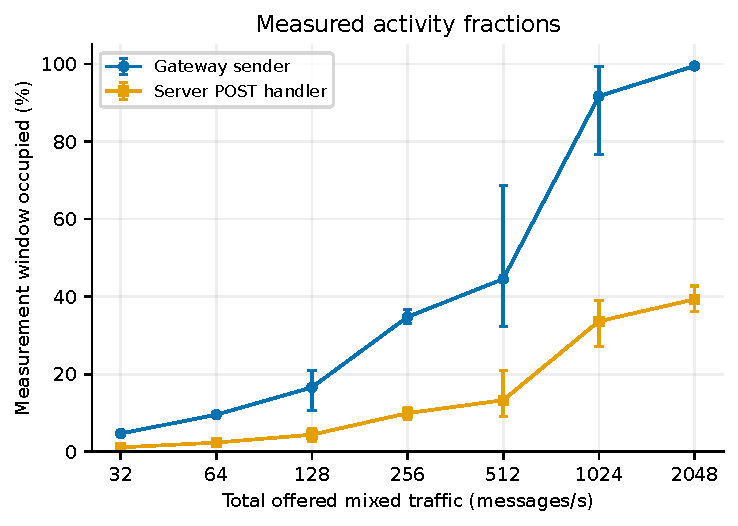
\includegraphics[width=0.88\linewidth]{figures/historical_fig6_busy_time.pdf}
\caption{Historical loopback sender and server-handler occupied fractions. Points average three runs; bars show minimum--maximum. These wall-time fractions differ from CPU use.}
\label{fig:e1r-historical-fig6-busy-time}
\end{figure}


At nominal 2,048/s the sender occupied 99.5\% of the window, versus 39.3\% for the server handler. Adding server workers alone cannot be assumed to remove a serial client-side restriction.

Every historical run at nominal 1,024 and 2,048 messages/s overflowed, but severity varied substantially. At the highest load, completed throughput ranged from 139.12--1,309.05 requests/s, and successful-message p95 ranged from 851.40--7,649.29 ms. Shared-host execution performance changed during the old sweep; the logs do not establish its cause. All repetitions remain included. Nominal 512/s was the highest tested old load with no overflow in all repetitions; it is an observed reference condition, not a fixed capacity claim.

\clearpage\subsection{Validation, calibration and reproducibility}

The revised cohort passed independent checks for all 35 runs. Its measurement windows contain 374,400 generated messages: 215,691 successful, 158,709 FIFO drops, 0 missing at the gateway, 0 request/HTTP errors and 0 unresolved after draining. These are measurement-cohort counts, excluding warm-up messages. FIFO drops are valid overload outcomes and do not imply a failed integrity check.

The validator recorded 0 warning entries across these runs. No per-run validation warnings were recorded.

The final validator inventories 0 infrastructure-invalid attempts outside the 35 valid runs. No infrastructure-invalid attempts were excluded from this final cohort.

Server-side connection identities show 1 TCP connection in 35 runs. Checks also cover unique IDs, source sequences and scheduled intervals, topic identities, FIFO order, stage ordering, response agreement, queue capacity, the one-request concurrency bound, configuration/code hashes, CPU calculations, deadline denominators and message conservation.

The host exposed 16 logical CPUs. The recorded middleware is \texttt{rmw\_fastrtps\_cpp}. Run creation spans 23 October 2026 at 04:59:20 UTC to 23 October 2026 at 05:42:51 UTC. The saved platform string, full-precision ISO timestamps and code/configuration provenance are available in the accompanying evidence file and original configurations.

\begin{table}[H]
\centering\small
\setlength{\tabcolsep}{4pt}
\begin{tabular}{lrrr}
\hline
Condition & Runs & Unloaded RTT (ms) & Bulk payload (Mbit/s) \\
\hline
Reference & 20 & 0.048--0.817 & 8,228.08--33,180.85 \\
Gateway +10 ms & 5 & 0.051--0.372 & 10,693.23--43,647.98 \\
Server +10 ms & 5 & 0.049--0.209 & 10,353.90--24,914.80 \\
Forward 2 Mbit/s & 5 & 0.056--0.090 & 1.91--1.92 \\
\hline
\end{tabular}
\caption{Pre-run path calibration ranges. RTT is the range of run-level unloaded ICMP mean RTTs. Bulk payload goodput comes from a separate TCP upload, not the REST application.}
\label{tab:e1r-calibration}
\end{table}


Each newly created path is verified before application measurement. Rate-limited calibration must deliver 70--120\% of the configured rate as TCP payload; the tolerance permits lower-layer overhead and finite-transfer effects. Unshaped calibration is a path sanity check, not a controlled bandwidth target. Qdisc/interface statistics, offload configuration and setup/cleanup commands are saved. Successful bulk calibration does not imply that serial mixed HTTP requests attain the same useful payload rate.

\begin{table}[H]
\centering\small
\setlength{\tabcolsep}{4pt}
\begin{tabular}{lrr}
\hline
Class & Configured Hz/source & Measured Hz/source range \\
\hline
command & 2 & 2.000 \\
status & 5 & 5.000 \\
odometry & 20 & 19.983--20.017 \\
sensor & 5 & 5.000 \\
\hline
\end{tabular}
\caption{Per-source generation-rate verification over all revised measurement windows. Individual source/run values are supplied in source\_rates.csv.}
\label{tab:e1r-rates}
\end{table}


Run-level p95 source scheduling lag ranged from 0.171--4.133 ms. The largest individual scheduling lag was 77.109 ms. Rate checks and scheduling lag should be read together: matching the total generated count does not demonstrate perfectly regular spacing.

\begin{table}[H]
\centering\small
\setlength{\tabcolsep}{4pt}
\begin{tabular}{lrrrrr}
\hline
Condition & Sources & Command & Status & Odometry & Sensor \\
\hline
Reference & 1 & 120 & 300 & 1,200--1,201 & 300 \\
Reference & 2 & 240 & 600 & 2,400--2,402 & 600 \\
Reference & 4 & 480 & 1,200 & 4,800 & 1,200 \\
Reference & 8 & 960 & 2,400 & 9,600 & 2,400 \\
Gateway +10 ms & 8 & 166--492 & 658--981 & 3,218--3,635 & 500--875 \\
Server +10 ms & 8 & 191--497 & 619--971 & 3,189--3,631 & 524--842 \\
Forward 2 Mbit/s & 8 & 171--284 & 552--668 & 2,288--2,692 & 547--607 \\
\hline
\end{tabular}
\caption{Successful latency samples per run: observed minimum--maximum across five repetitions. These support the class percentiles and are not pooled sample sizes. Exact generated/successful counts and mean run-level p95/p99 are supplied in class\_samples.csv.}
\label{tab:e1r-samples}
\end{table}


The main analysis emphasises p95. A single source produces only 120 commands per 60 s run, so its p99 is supported by very few upper-tail observations. It should not be interpreted as a precise tail guarantee. The sample table makes reduced successful sample counts under overload explicit.

35 application packet captures were recorded. Kernel capture-drop counts were available for 35 captures and totalled 0. These describe capture loss, not network loss or retransmissions. Application logs supply pre-transmission queue and end-to-end measurements; this report does not infer TCP retransmission counts from capture-drop counters.

Independent TCP stream reassembly reconciled 266,486 HTTP requests and the same number of responses with the server logs, including warm-up, measurement and drain exchanges. The checker verified message identifiers and order, request-body byte totals, a single connection per run and complete captured streams. These all-run exchange counts have a different time scope from the measurement-cohort totals above.

\subsection{Conclusions and limits}

The completed evidence separates actual source-node scaling from aggregate rate scaling and distinguishes controlled restrictions through stage timestamps. The revised source sweep measures 1--8 actual ROS 2 nodes feeding one client. Its diagnostics quantify the effects of gateway waiting, server waiting and forward bandwidth under an unchanged eight-source workload. The historical high-load sweep supplies complementary evidence of queue growth, deadline failure and repeat variability. Neither cohort establishes multi-client scalability; independent per-source gateways require a different experiment.

All processes share one host and kernel. Virtual networking and sleep-based delays isolate mechanisms without reproducing every property of independent machines, physical radio links or CPU-intensive services. Five repetitions reveal a finite observed spread, not a confidence interval; host scheduling and runtime conditions can still change performance. The network diagnostic changes forward bandwidth, without independently varying propagation delay or loss. These results provide a baseline for later scheduling, transport and topology experiments rather than a universal capacity limit or deployment safety claim.

\clearpage
\appendix
\section{Supplementary Historical Loopback Evidence}

This appendix contains the five additional plots from the historical 21-run cohort. It does not add new measurements or pool the old loopback results with the revised veth experiment. Historical rate-sweep points average three run-level statistics and error bars show minimum--maximum, not confidence intervals.

\subsection{Application payload goodput}

Payload bytes in successful completions inside the 60 s window were summed, converted to bits and divided by the window duration. Metadata, protocol headers and acknowledgement responses are excluded. The dashed line denotes configured payload offered across all classes.

\begin{figure}[H]
\centering
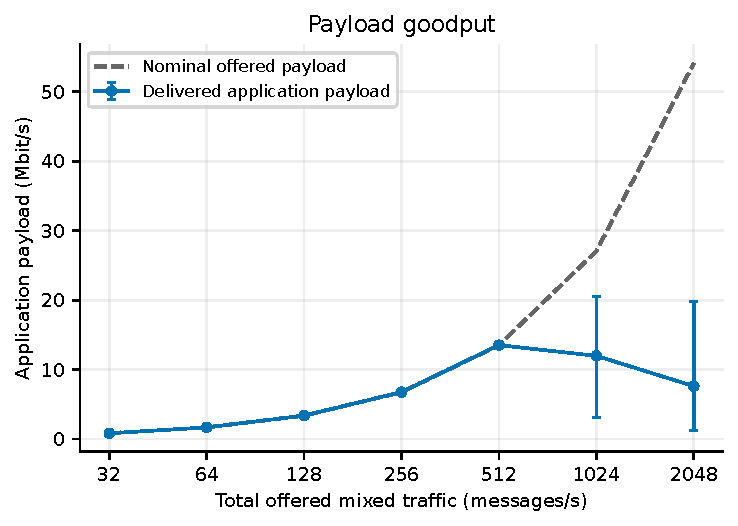
\includegraphics[width=0.88\linewidth]{figures/historical_appendix_goodput.pdf}
\caption{Historical loopback application payload goodput. Points average three runs; bars show minimum--maximum. The horizontal rate includes all four classes.}
\label{fig:e1r-historical-appendix-goodput}
\end{figure}


Goodput averaged 13.53 Mbit/s at nominal 512 messages/s and 7.62 Mbit/s at nominal 2,048 messages/s, despite 54.1184 Mbit/s of configured payload offered at the latter load. Useful payload and completed request count answer different questions when message sizes and the delivered class mix differ.

\subsection{Admission loss under overload}

Each run's FIFO-drop count was divided by its generated measurement-cohort count; the plot averages those three fractions. This differs from pooling all messages before computing a fraction, although the reported rounded values are close.

\begin{figure}[H]
\centering
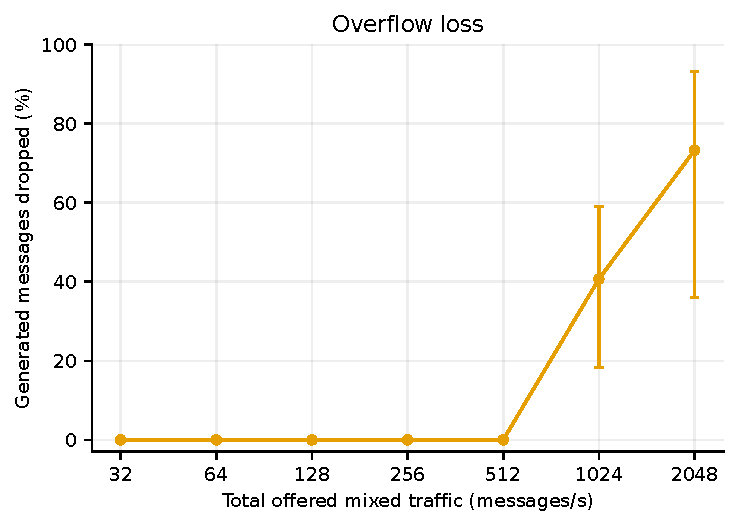
\includegraphics[width=0.88\linewidth]{figures/historical_appendix_drops.pdf}
\caption{Historical FIFO admission-drop percentage versus total offered mixed traffic. Points average three run fractions; bars show minimum--maximum.}
\label{fig:e1r-historical-appendix-drops}
\end{figure}


Mean per-run FIFO-drop percentages were 40.68\% at nominal 1,024 messages/s and 73.27\% at nominal 2,048/s. These are application admission losses. The rejected messages were never sent as HTTP requests.

\subsection{Queue evolution in selected repetitions}

The piecewise-constant waiting-queue state was sampled every 100 ms during repeat 1 at nominal 512, 1,024 and 2,048 messages/s. The same repeat index is selected at every load; this is not a best-run selection. Repeat indices do not indicate chronological run order.

\begin{figure}[H]
\centering
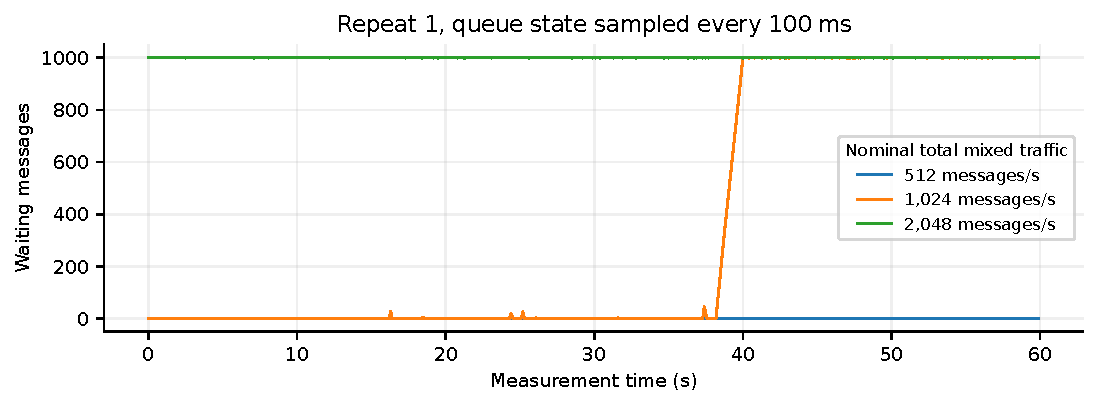
\includegraphics[width=0.88\linewidth]{figures/historical_appendix_queue_trace.pdf}
\caption{Historical waiting-queue traces for repeat 1 of the three highest nominal total traffic rates. Legend values are messages/s across all four classes.}
\label{fig:e1r-historical-appendix-queue-trace}
\end{figure}


The time traces expose whether backlog is present throughout a measurement or develops within it. A whole-run mean cannot distinguish those temporal patterns. These three examples should not be assumed to represent every repetition.

\subsection{CPU variation within one run}

For repeat 1 at nominal 1,024 messages/s, cumulative CPU counters were interpolated at consecutive 10 s boundaries. CPU-time differences were divided by elapsed wall time, with 100 percent representing one logical CPU. Lines connect bin averages rather than instantaneous readings.

\begin{figure}[H]
\centering
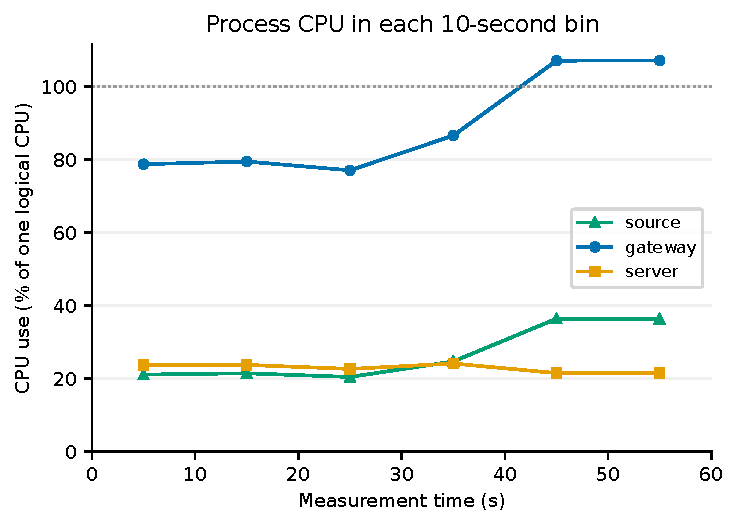
\includegraphics[width=0.88\linewidth]{figures/historical_appendix_within_run_cpu.pdf}
\caption{Historical process CPU in 10 s bins of repeat 1 at nominal 1,024 total messages/s. No repeat error bars are attached to a single-run trace.}
\label{fig:e1r-historical-appendix-within-run-cpu}
\end{figure}


Gateway CPU changed from 78.8\% in the first 10 s bin to 107.2\% in the final bin. This demonstrates changing within-run execution behaviour at a constant configured offered rate; it does not establish a thermal, scheduling or software cause.

\subsection{Queue variation within the same run}

Queue-state intervals were clipped to the same 10 s boundaries and integrated within each bin. The six duration-weighted bin means reproduce the validated whole-window occupancy. The dashed line is the 1,000-message waiting capacity.

\begin{figure}[H]
\centering
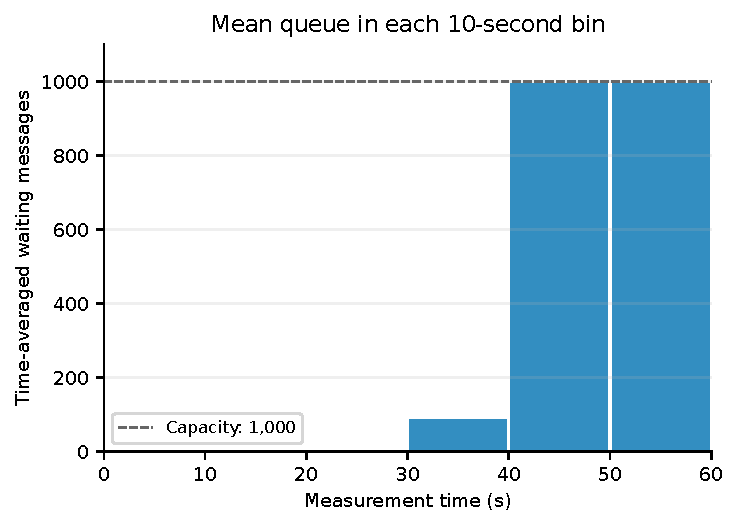
\includegraphics[width=0.88\linewidth]{figures/historical_appendix_within_run_queue.pdf}
\caption{Historical mean FIFO occupancy in 10 s bins of the same repeat-1 run at nominal 1,024 total messages/s.}
\label{fig:e1r-historical-appendix-within-run-queue}
\end{figure}


The first-bin mean queue was 0.95 messages and the final-bin mean was 999.63. Reading this alongside the CPU trace reveals coincident changes in activity and backlog, without identifying a causal explanation.

\end{document}
